\documentclass[draft=false]{oblivoir}
\author{Moon Il-chul \\ \href{mailto:icmoon@kaist.ac.kr}{icmoon@kaist.ac.kr} 
   \and Shin Yongjin \\ \href{mailto:dreimer@postech.ac.kr}{dreimer@postech.ac.kr} }
\setcounter{chapter}{16}
\title{Chapter 16. Recurrent Neural Network}
\usepackage{indentfirst}
\usepackage{graphicx}
\usepackage[draft=false]{hyperref}
\usepackage{amsmath}
\usepackage{amssymb}
\usepackage{amsfonts}
\usepackage[]{algorithm2e}
\usepackage{geometry}
\usepackage{algorithm}
\usepackage{algpseudocode}
\hypersetup{pdfborder={0 0 0}}
\renewcommand{\theequation}{\thechapter.\arabic{equation}}
\newlength\myindent
\setlength\myindent{5em}

\begin{document}

\maketitle
\tableofcontents

% 1. -----------------------------------------------------------------
\section{Recurrent Neural Network}

% 1.1 -----------------------------------------------------------------
\subsection{Overview}
이전 강의에서 다루었던 Fully Connected Network는 네트워크를 구성하는 모든 뉴런 사이에 연결이 이루어질 수 있다. 이는 네트워크가 유연하다고 볼 수도 있지만 연결이 많아지는 것은 곧 매개변수(Parameter)의 개수가 증가함을 의미한다. 매개변수의 수가 증가할 수록 데이터셋이 주어졌을 때, 모델이 참값을 가질 수 있는 확률은 떨어지게 된다. 따라서 모델이 유연하다는 것이 장점이 될 수도 있으나, 특정한 문제 상황을 반영하기 위해 너무 많은 연결이 이루어져야 한다면 모델을 학습시키기 용이하지 않다는 단점을 가지기도 한다. 따라서 특정한 문제를 잘 표현할 수 있도록 뉴럴 네트워크의 구조 자체를 변형시키는 접근이 필요하다. 이 변형의 방법 중의 하나로 RNN(Recurrent Neural Network)는 시간의 흐름(Time flow)이라는 문제상황을 반영하는 모델이다.

% 1.2 -----------------------------------------------------------------
\subsection{Recurrent Neural Networks for Various Domains}

\begin{figure}[ht] \centering 
  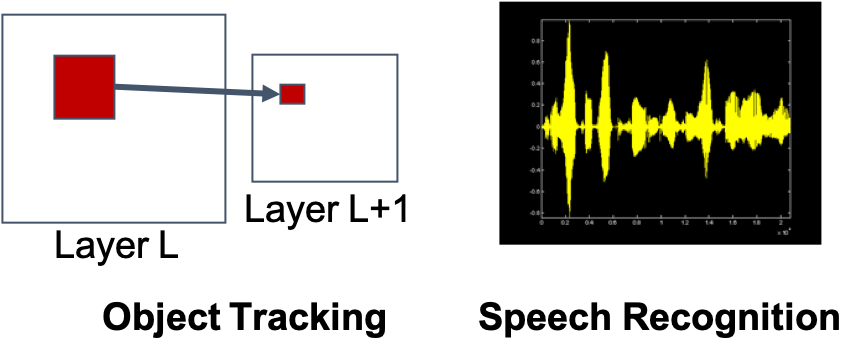
\includegraphics[scale=0.5]{fig1.png}
  \caption{분야}
  \label{fig:16-1}
\end{figure}

다음과 같은 세 가지 분야는 시간의 흐름(Time flow)을 지닌 문제를 다루는 대표적인 분야이다. 첫째로 움직이는 물체를 따라가는 Object tracking 분야가 있다. 예를 들어, 화면 속에 날아가는 비행기의 위치를 시간의 흐름에 따라 예측을 하는 문제가 있다. 둘째로 번역 Language Translation 분야가 있다. 예를 들어, 'Hello'는 'H', 'e', 'l', 'l', 'o'라는 문자가 시간에 따라 흘러가는데, 이를 어떻게  '안', '녕', '하', '세', '요' (즉, '안녕하세요')으로 번역을 할 것인가 라는 문제가 있다. 세번째로 음성 인식 Speech Recognition이라는 분야가 있다. 화자가 발생하는 소리에서 파형이 시간의 흐름에 따라서 형성되므로 이를 분석하여 어떤 말을 하는지 알아낼 수 있다. RNN에서 'Recur'이 의미하는 바는  '\textit{다시 발생하다, 순환하다}' 이다. 따라서 RNN은 시점 t의 네트워크 구조를 시점 t+1에서도 \textit{다시 사용하는 것}이라 할 수 있다. 

\begin{figure}[ht] \centering 
  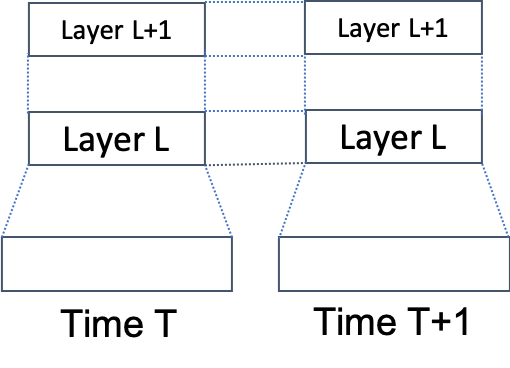
\includegraphics[scale=0.7]{fig2.png}
  \caption{Recurrent Neural Network}
  \label{fig:16-2}
\end{figure}

% 1.3 -----------------------------------------------------------------
\subsection{Detour: Multiple Layers of Neural Network}

\begin{figure}[ht] \centering 
  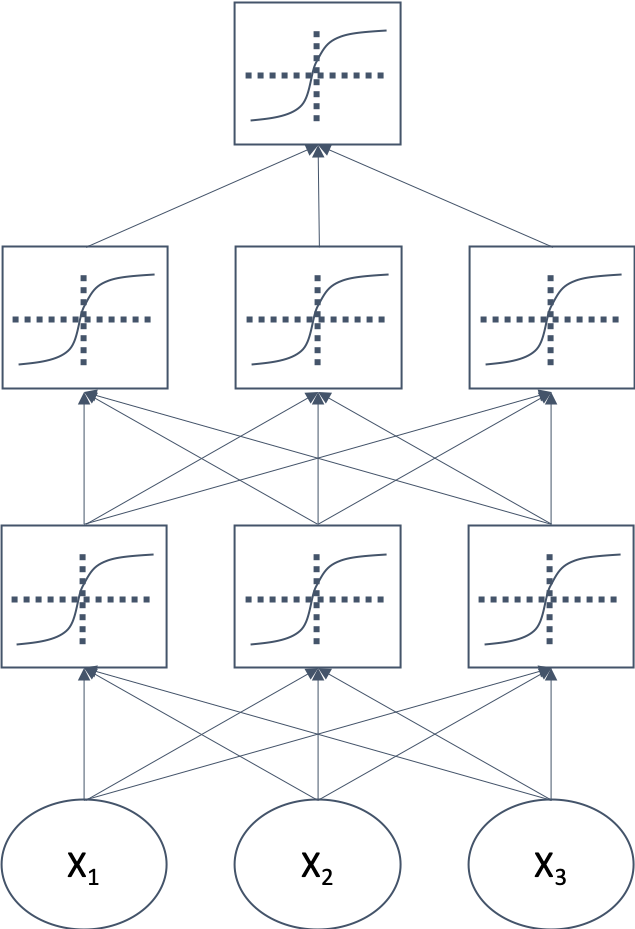
\includegraphics[scale=0.5]{fig3.png}
  \caption{Fully Connected Neural Network}
  \label{fig:16-3}
\end{figure}
 
 Recurrent Neural Network의 구조와 학습 방법에 대해서 자세하게 다루어보기 이전에 Multiple Layers of Neural Network의 구조를 간단히 되짚어 보도록 하겠다. 위의 그림 \ref{fig:16-3}에서 Output layer의 Activation fucntion은 $h^{L+1}(x) = o (a^{L+1}(x)) = f(x)$와 같이 정의되어 있으며, Hidden Layers는 두 개의 층으로 형성되어 있다. 가장 아래는 Input layer로 되어 있다. 개별 Layer는 Activation function으로 Sigmoid function을 이용하고 있으며, 최근에는 Sigmoid function이 아니더라도 Softplus, Relu 등 다양한 Activation Function을 활용하여 네트워크를 구성한다. 더불어 상위 단계에서는 꼭 하나의 Output만 만들어 내는 것이 아니라 다수의 Output을 만들어 낼 수도 있으며, Softmax function을 통해 Category정보에 대한 분류문제도 해결할 수 있다. 
 
 % 1.4 -----------------------------------------------------------------
\subsection{Detour: Backpropagation}
 
 \begin{figure}[ht] \centering 
  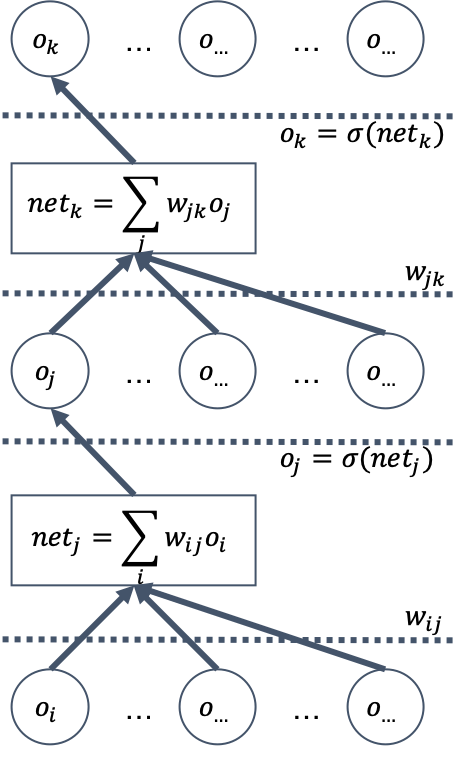
\includegraphics[scale=0.6]{fig4.png}
  \caption{Fully Connected Neural Network}
  \label{fig:16-4}
\end{figure}
 
 이러한 다수의 Layers를 가지는 네트워크를 가정한 상황에서 학습을 어떻게 하는지 다시 복습을 해보도록 하자. 뉴럴 네트워크에서 Parameter는 그림 \ref{fig:16-4}에서 Layer간의 연결(connection) 을 만들어 주는 선형결합식의 계수인 $w_k$를 일컫는다. 이에 대한 학습은 Backpropagation에 의해 이루어지게 되는데, 실제 값과 얼마나 차이가 나는지에 대한 정보인 $\delta$ Signal이 상단의 Layer으로부터 하단까지 전달되는 과정이라 할 수 있겠다. 이렇게 한번 만들어진 $\delta$ Signal들을 업데이트하면서 매 Layer마다 전파가 가능하다는 것이 Backpropagation의 핵심 알고리즘이라 할 수 있겠다.

% 1.5 -----------------------------------------------------------------
\subsection{Modeling Temporal Data with Neural Network}
CNN(Convolution Neural Network) 구조는 지역적인 정보(local Information)을 반영할 수 있지만, 시간의 흐름에 따른 모델링이 불가능하다는 한계점을 지니고 있다. 따라서 앞서 언급하였듯이 RNN은 시계열 데이터를 반영할 수 있도록 네트워크의 구조가 고안되었다. RNN을 한마디로 표현하자면 다음의 수식과 같이 표현할 수 있다.
\begin{equation}
	h_t = \sigma (Uh_{t-1} + Wx_{t}+b)
\label{eq:16-1}
\end{equation}
수식(\ref{eq:16-1})의 $h_t$는 현재 시점 t에서의 잠재 정보(Hidden Information)라고 할 수 있다.  $h_t$는 이전 시점인 t-1에서 넘겨진 $h_{t-1}$으로부터 영향을 받을 뿐만 아니라 현재 시점 t에서 주어지는 값 $x_t$ 에 의해서도 영향을 받게 된다. 이것은 HMM(Hidden Markov Model)과 구조적으로 동일하다. 

\begin{figure}[ht] \centering 
  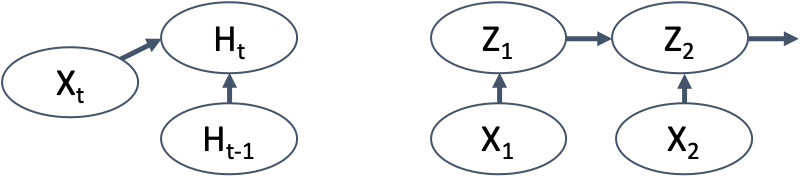
\includegraphics[scale=0.7]{fig5.png}
  \caption{RNN vs HMM}
\label{fig:16-5}
\end{figure}

위의 그림 \ref{fig:16-5}의 왼쪽은 시간에 따라서 잠재 변수 $z_t$가 관측값 $x_t$를 만들어 낸다라는 것을 표현하고 있다. 이 때, 잠재 변수 $z_t$는 $x_t$가 영향을 미치고, $z_{t}$와 $z_{t+1}$ 는 서로 영향을 미친다. 이는 Generative Process 관점에서 확률 모델을 활용한 정보의 생성 과정이라 할 수 있다. 따라서 확률 모델(Graphical Modeling)의 관점에서 아래 수식(\ref{eq:16-2})과 같이 표현을 할 수 있다.

\begin{equation}
	p(z_1) \times p(z_2|z_1) \times p(x_1|z_1) \times p(x_2|z_2)
\label{eq:16-2}
\end{equation}

반면, 그림 \ref{fig:16-5}의 오른쪽은 Discriminative의 관점에서 $x_t$와 $h_{t-1}$이 어떻게 $h_t$를 설명하는데 사용될 수 있을지를 표현하고 있다. 현재 단계에서는 HMM에서 표현한 것과 같이 확률로 관계를 표현하기는 힘들지만, Logistic Regression을 표현하는 수식(\ref{eq:16-3})과 비슷하게 이를 이해해볼 수 있다. 

\begin{equation}
	p(Y|X) = \frac{1}{1+(1+e^{-X \theta})}
\label{eq:16-3}
\end{equation}

여기서 Exponential 속에 $X$와 $\theta$의 선형결합이 이루어진 것을 확인할 수 있는데, 수식(\ref{eq:16-2})의 $Uh_{t-1}+Wx_{t}+b$의 선형결합이 이와 같은 역할을 한다고 할 수 있겠다. 따라서 이것은 Discriminative 기반으로 시간의 흐름을 모델링한다고 볼 수 있겠다. 한편, 수식(\ref{eq:16-2})의 $p(z_{t}|z_{t-1})$의 부분이 수식(\ref{eq:16-1})에서의 $h_t = \sigma(Uh_{t-1} + \beta)$와 유사함을 확인할 수 있다. 따라서 시간의 흐름을 표현하기 위해 이전 시점의 정보를 이용하여 다음 시점의 정보를 표현한다는 점에서 구조적으로는 HMM과 RNN의 유사점을 확인할 수 있다.\par

\begin{figure}[ht] \centering 
  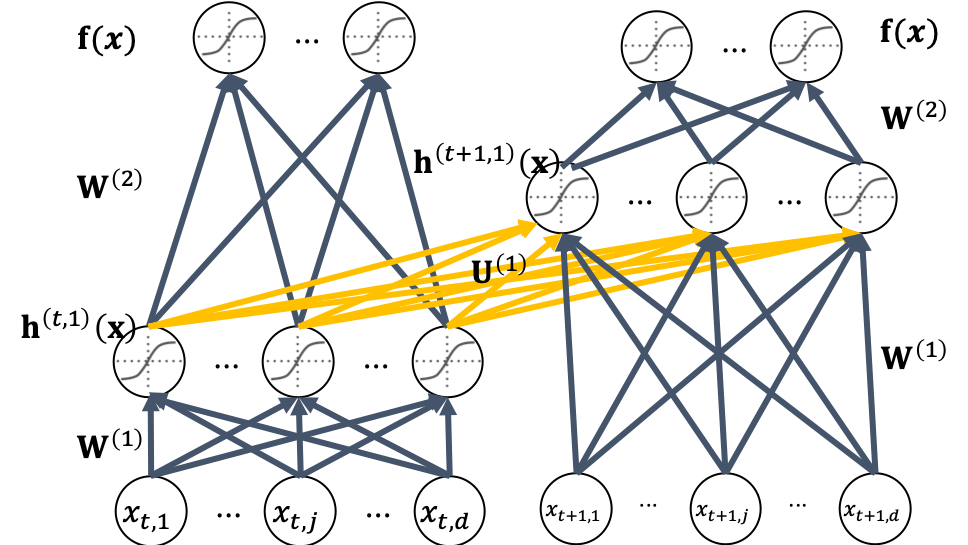
\includegraphics[scale=0.6]{fig6.png}
  \caption{RNN}
  \label{fig:16-6}
\end{figure}

뉴런 관점에서 RNN을 바라보면 그림(\ref{fig:16-6})과 같이 표현할 수 있는데, Fully Connected의 그래프가 \textit{다시 발생하면서(Recur)} 사용된다. $x$라고 하는 정보가 들어온다고 할 때, Hidden layer가 하나가 존재하여 $h_1$을 만들어내고, 이 Hidden layer가 Output layer에 연결이 된다. 만약 RNN이 아닐 경우 (즉 위의 그림에서 노란 연결선들이 없을 경우에는) 좌측 네트워크와 우측의 네트워크 2개로 나뉘어지게 된다. 이 경우에는 두 네트워크는 다른 네트워크가 된다. 따라서 매 시점마다 다른 Hidden Layer가 생성된다고 할 수 있겠다. 하지만 RNN 구조에서는 노란 연결선$(U)$을 추가하면서 이전 시점의 Hidden layer의 정보$(h_{t-1})$를 다음 시점의 Hidden layer의 정보$(h_t)$에 Fully Connect되게 한다. 이때, $W$와 $U$는 매 시점에 새로이 생겨나는 것이 아니라 \textit{반복하여 사용}된다라는 점이다. 따라서 시점 t-1일 때 사용되었던 $W$와 $U$는 시점이 t일 경우에도 동일하게 사용된다. 이렇게 RNN은 변수(parameter)를 반복하여 사용하는 구조이기 때문에 이 Layer 구조를 다음 그림(\ref{fig:16-7})과 같이 표현을 할 수도 있겠다.

\begin{figure}[ht] \centering 
  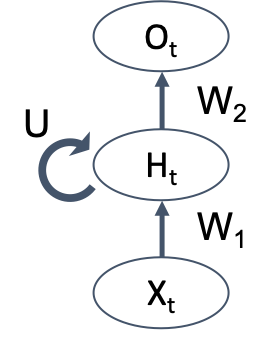
\includegraphics[scale=0.7]{fig7.png}
  \caption{RNN}
  \label{fig:16-7}
\end{figure}

% 1.6 -----------------------------------------------------------------
\subsection{Variant of Recurrent Neural Network}
앞서 살펴보았듯이  RNN은 이전 시점의 Hidden Layer의 정보를 선형 결합$(Uh_{t-1})$을 통해 다음 시점으로 넘겨주는 구조라고 할 수 있겠다. 이를 다양한 형태로 확장할 수 있다. 

\begin{figure}[ht] \centering 
  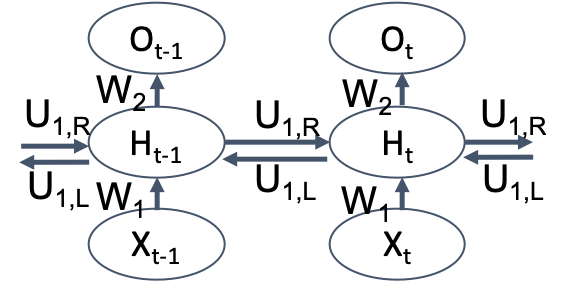
\includegraphics[scale=0.7]{fig8.png}
  \caption{Bidirectional RNN}
  \label{fig:16-8}
\end{figure}

첫째로 Bidirectional RNN구조가 있다. 이 구조는 그림(\ref{fig:16-8})과 같이 $H_{t-1}$의 정보를 $U_{1,R}$에 의해 다음 시점 $H_t$으로 연결해 줄 수 있지만, $U_{1,L}$에 의해서 $H_t$의 정보를 이전 시점인  $H_{t-1}$으로도 연결을 해줄 수 있다. 개체명 인식(Named entity recognition), 형태소 분석(POS tagging) 등을 할 때 시간을 거슬러 올라오는 구조를 활용할 수 있다. 예를 들어, '\textit{My name is Michael}.'이라고 하는 문장을 볼 때,  '\textit{My}'와 '\textit{Michael}'은 동일한 인물을 가리키는데 '\textit{Michael}'을 표현하기 위해서 두 단계 이전에 '\textit{My}'라는 단어를 사용하게 되었다. 이러한 구조를 분석하기 위해서 Bidirectional RNN이 사용될 수 있다.\par

\begin{figure}[ht] \centering 
  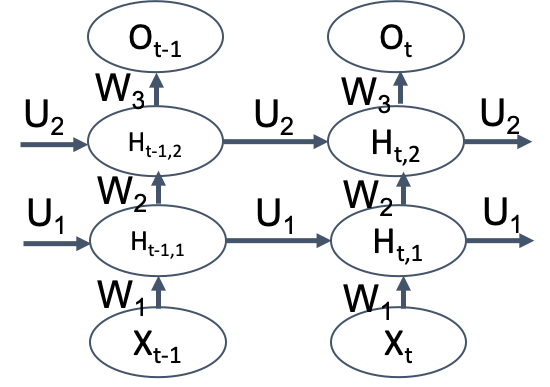
\includegraphics[scale=0.7]{fig9.png}
  \caption{Deep RNN}
  \label{fig:16-9}
\end{figure}

둘째로 Deep RNN의 형태로 만들 수 있는데, 이 구조는 위 그림(\ref{fig:16-7})과 같이 RNN에서 겹겹의 층을 더 추가하여 만든 것이라 할 수 있다. 즉, 가장 아래쪽 Layer에서 $U_1$ 이 시간의 흐름을 전달하고 그 다음 Layer는 $U_2$가 존재하여 아래 Layer에서 전달된 정보들을 다시 시간의 흐름에 따라 다음 시점으로 전달이 가능하도록 한다. \par

\begin{figure}[ht] \centering 
  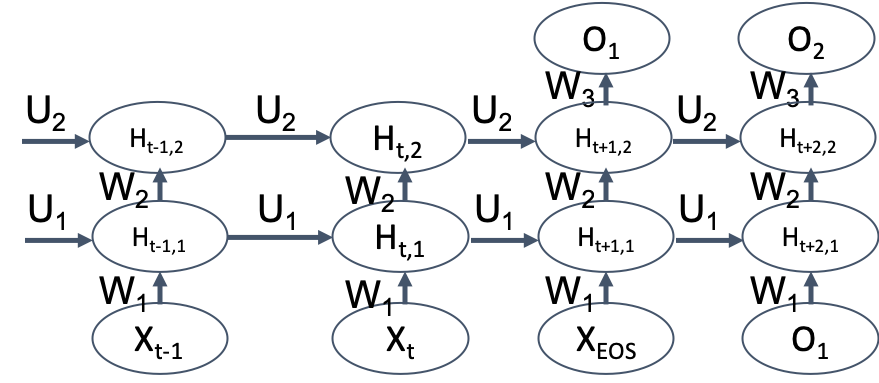
\includegraphics[scale=0.7]{fig10.png}
  \caption{그림 Deep seqeuence2sequence}
  \label{fig:16-10}
\end{figure}

셋째로 Deep Sequence-to-Sequence RNN 구조는 그림(\ref{fig:16-10})과 같이 표현이 가능하다. 이 구조의 앞 부분은 기존 모델과 달리 Output이 존재하지 않는다라는 차이점이 하나 존재한다. 즉, Output 없이 시간에 따라 입력된 값$(x_t)$의 함축적인 정보$(H_{t,1}, H_{t,2})$만을 전달한다. 반면, 뒷 부분은 디코딩이 시작된다라는 입력값인  \textit{GO}가 입력되면 앞 부분에서 전달받은 Hidden Layer의 정보를 통해 Output을 생성하게 된다. 이러한 구조는 특히 기계번역(Machine Translation) 분야에서 활발하게 사용이 된다. 

% 1.7 -----------------------------------------------------------------
\subsection{Detour: Vanishing Gradient Problem}
그러나 RNN 역시 그 구조적인 특징으로 인하여 Vanishing Gradient Problem이 발생할 수 밖에 없다. Logistic function을 떠올려 보면 다음과 같은 수식(\ref{eq:16-4})으로 나타낼 수 있음을 기억할 것이다.

\begin{equation}
	f(x) = \frac{1}{1+\exp{(-x)}}
	\label{eq:16-4}
\end{equation}

앞서 언급하였듯이, Backpropagation을 수행하기 위해서는 $\delta$ signal이 필요하게 되고, 이를 구하기 위해서는 위의 수식을 미분해야만 한다는 것을 독자들을 이미 알고 있을 것이다. 이를 계산을 하면 다음과 같이 표현할 수 있다.

\begin{equation}
    \begin{split}
        \frac{d}{dx}f(x) & = \frac{d}{dx}(1+e^{-x})^{-1} \\
        & = e^{-x}(1+e^{-x})^{-2} \\
        & = f(x)(1-f(x))\\
    \end{split}
    \label{eq:16-5}
\end{equation}

그러나 Logistic function $f(x)$는 0과 1사이에서 존재하는 함수($max \frac{d}{dx}f(x) = \frac{1}{4}$)이므로 $1-f(x)$역시 0과 1 사이에 존재하게 된다. 따라서 $f(x)$와 $1-f(x)$의 곱셈의 결과 역시 1을 넘지는 못하게 되고 0에 가까워질 수 밖에 없다. 

\begin{equation}
 	\delta_j = o_j (1-o_j ) \sum_{k}\delta_{k}w_{jk}
 	\label{eq:16-6}
 \end{equation}
 
그러나 $\delta$ signal을 만드는 과정의 수식(\ref{eq:16-6})을 살펴보면 $o_j (1-o_j)$을 구하기 위한 값이 Logistic function의 미분 값과 동일하다는 것을 확인할 수 있다. 따라서 0과 1 사이의 값이 $\delta$ signal이 계속해서 곱하여질 수 밖에 없고 0에 수렴해질 수 밖에 없다고 유추할 수 있다. 이 사실은 RNN에서 사용되는 Layer의 수와 Sequence의 길이가 길어질수록 $\delta$ Signal의 크기가 작아져 학습에 어려움이 발생한다는 것을 의미한다. CNN에서는 이러한 Vanishing Gradient 문제를 해결하기 위해서 Activation function에 변화를 가한 반면, RNN에서는 다른 형태의 해결책을 활용하게 된다. 즉, 다수의 Sequence와 Layer를 거쳐야 하는 경우에는 $\delta$ signal이 너무 작은 값을 가지는 것을 방지하기 위해서 \textit{Gating Mechanism}을 도입하여 LSTM(Long Short Term Memory)과 같은 구조를 만들게 된다. 
 
% 2. -----------------------------------------------------------------
\section{LSTM and GRU}

% 2.1 -----------------------------------------------------------------
\subsection{Gating Mechanism in Deep Neural Network}

\begin{figure}[ht] \centering 
  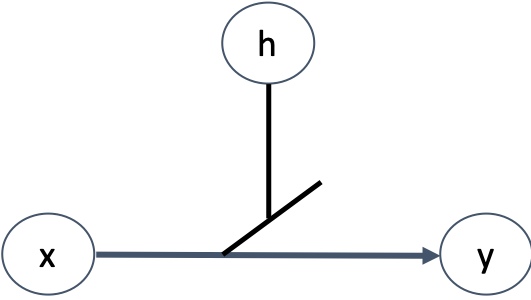
\includegraphics[scale=0.5]{fig11.png}
  \caption{Gating Mechanism}
  \label{fig:16-11}
\end{figure}

Gating Mechanism은 위 그림(\ref{fig:16-11})과 같이 마치 스위치처럼 작동을 하여 정보의 흐름을 제어한다. X에서 Y로 정보가 전달된다고 할 때, $h$라는 스위치가 존재한다고 생각해보자. $h$가 눌러지지 않을 경우에는 X에서 Y로 정보가 전달될 수 있게 된다. 그러나 $h$가 충분히 눌러질 경우에는 X에서 Y로 정보가 전달되지 않게 된다. 스위치 $h$는 눌러지는가, 안 눌러지는가로 결정이 될 수 있으므로 0과 1사이에서 결정되는 Logistic Regression의 Sigmoid function으로 생각을 할 수 있다. 즉, Soft Switch를 만든다라고 할 수 있다.

\begin{equation}
  y = 
  \left\{
    \begin{array}{ll}
      x \quad if \quad h=1\\
      0 \quad if \quad h=0\\
      h\times x, \quad otherwise\\
    \end{array}
  \right.
  \label{eq:16-7}
\end{equation}

위 수식(\ref{eq:16-7})과 같이 $h$가 1일 경우에는 X의 정보가 온전히 Y로 전달되는 반면, $h$가 0일 때에는 X의 정보가 Y로 전혀 전달되지 않는다. 그러나 $h$가 0과  1사이의 값이 경우에는 $h$ 값 만큼의 가중치만큼 X에 곱해져서 전될됨을 알 수 있다. 

\begin{equation}
	y = x \odot h
	\label{eq:16-8}
\end{equation}

이를 수식적으로 가능케 하는 것은 Multiplicative gates라 할 수 있으며 Element-wise하게 연산이 되어 위의 수식(\ref{eq:16-8})과 같이 나타낼 수 있다 (따라서 이 경우 $h$는 $x$와 같은 차원을 가진 벡터형식이어야만 한다). 이런 Gating Mechanism을 RNN에 적용시켜 시간의 흐름에 따라 정보의 전달 여부를 반영할 수 있게 되었는데, 이와 같은 모델 중 하나가 LSTM이다.\par

% 2.2 -----------------------------------------------------------------
\subsection{Long Short Term Memory}
기존의 RNN 구조에서는 시간의 흐름에 따라 하나의 정보인 $h_t$만 전달되는 반면, LSTM(Long Short Term Memory)에서는 두 개의 정보($h_t$와 해당 시점의 셀(cell)의 상태(state) 정보를 담고 있는 $C_t$)로 나뉘어 전달된다.  $C_t$는 LSTM에서 새로 등장하게 된 값으로서 상대적으로 긴 시간의 정보 전달을 담당하는 역할을 한다. 

\begin{figure}[ht] \centering 
  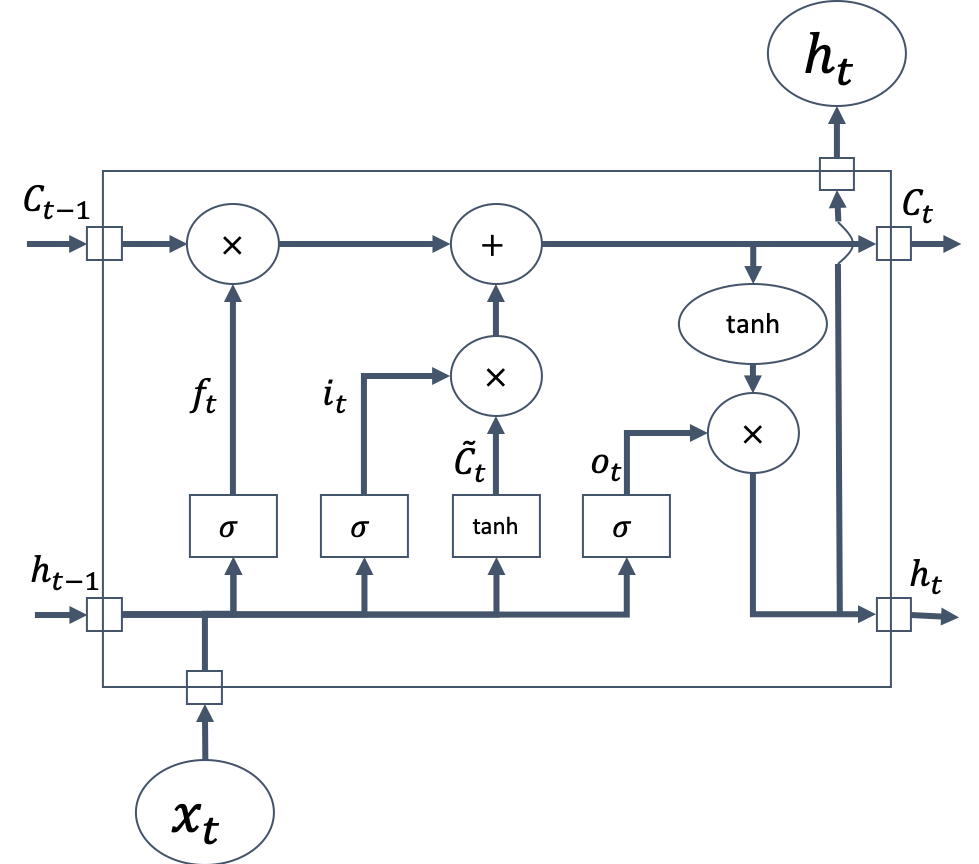
\includegraphics[scale=0.5]{fig12.png}
  \caption{그림 LSTM}
  \label{fig:16-12}
\end{figure}

위의 그림(\ref{fig:16-12})처럼 LSTM의 셀(cell)은 기존 RNN 셀(cell) 보다 복잡하게 구조화되었다. 이 때 $f_t$는 $\otimes$으로 연결이 되는데, 이 $\otimes$가 Gating Mechanism이 적용된 Multiplicative Gates로서 Element-wise하게 연산이 이루어진다. 그림에서 보듯이 3개의 $\otimes$ 모두 Gating Mechanism이 적용되는 부분이라 이해하면 되겠다. 아래 수식을 통해 LSTM 구조가 어떻게 여러 개의 Gating Mechanism을 활용하여 정보 전달 여부를 조절하는지를 확인할 수 있다. 

\begin{equation}
	\begin{split}
		f_t &= \sigma (W_f [h_{t-1}, x_t] + b_f)\\
	\end{split}
	\label{eq:16-9}
\end{equation}

먼저, Forgetting Process인 $f_t$는 이전 시점까지의 정보 중 얼마만큼을 잊을 것인가를 결정하는 역할을 담당한다. 즉, 새로운 들어오는 정보를 기억하기 위해서 지금 오래된 정보 중 들어오는 정보와 관련이 없는 부분을 삭제하는 것이라 이해할 수 있겠다. RNN과 유사하게 이전 시점의 $h_{t-1}$과 현재 시점의 $x_t$이 합쳐진(Concatenate) 값이 $W_f$, $b_f$와 선형 결합으로 이루어진다. 이는  $h_{t-1}$과 현재 시점의 $x_t$으로 셀의 상태(cell state) $c_{t-1}$ 중 어떤 것을 $c_t$으로 흘려보내지 않을 것인지를 결정하는 것이다.\par

\begin{equation}
	\begin{split}
		i_t &= \sigma (W_i [h_{t-1}, x_t] + b_i)\\
        \tilde{C_t} & = tanh (W_c [h_{t-1}, x_t] + b_c)\\
	\end{split}
	\label{eq:16-10}
\end{equation}

반면, Remembering Process인 $i_t$와 $\tilde{C_t}$에서는 앞으로 어떤 정보를 기억할 것인가를 결정하는 역할을 담당한다. 이때 $\oplus$는 $C_{t-1}$에서 $C_t$으로 넘어갈 때 정보를 추가하는 역할을 한다. 어떤 정보를 추가할 것인지는 스위치처럼 작동되는 $i_t$와 현재 시점의 정보 $\tilde{C_t}$의 $\otimes$연산을 통해 결정된다. $i_t, \tilde{C_t}$는 $f_t$와 유사하게 $h_{t-1}$과 $x_t$에 의해서 결정이 된다. 주목할만한 점은 다른 Sigmoid function과는 다르게 $\tilde{C}_t$는 Sigmoid function으로 $tanh$를 가진다는 점이다. 이는 Logistic function과는 달리 $tanh$의 공역이 -1부터 1사이에 존재하기 때문에 $\oplus$으로 뺄셈 연산까지 할 수 있기 때문이다. 이러한 과정을 통해 선별적으로 선택된 현재 시점의 정보를 셀 상태(cell state)에 추가해줄 수 있게 된다.\par

\begin{equation}
	\begin{split}
		C_t & = f_t \odot C_{t-1} + i_{t} \odot \tilde{C_{t}}\\
        o_t & = \sigma(W_{o}[h_{t-1}, x_t] + b_o)\\
        h_t & = o_t \odot tanh(C_t)\\
	\end{split}
	\label{eq:16-11}
\end{equation}

위와 같이 형성된 Forgetting Process와 Remembering Process를 Multiplicative Gate를 통해서 $C_{t-1}$에서 $C_t$으로 정보를 전달하여 Output 중 하나를 결정지을 수 있다. 앞에서도 언급했듯이 이 $C_t$는 장기 기억을 담당하고 LSTM은 단기 기억을 담당하는 $h_t$ 역시 Output으로 생성을 해내야만 한다. 이러한 과정은 Output Process라고 하며, $o_t$와 $h_t$에 의해 결정된다. $o_t$는 $f_t$나 $i_t$와 마찬가지로 스위치 역할을 담당하게 된다. 즉, 수식을 해석하면 $tanh$에 의해 변형된 $C_t$의 값이 $h_t$으로 전달되고, 이 정보의 흐름을 $o_t$가 통제한다는 것이다. $C_t$는 장기적인 관점에서 흘러가는 정보를 함축하고 있으나, $h_t$는 시점마다의 특징을 함축하고 있는 정보라 할 수 있겠다. $h_t$는 RNN과 동일하게 다음 시점으로 전달되는 동시에 해당 시점의 Output으로 사용된다.

% 2.3 -----------------------------------------------------------------
\subsection{Pros and Cons of LSTM}
LSTM은 셀의 상태(cell state)에서 $\otimes$ gate와 $\oplus$으로만 연산이 이루어지기 때문에 미분 과정에서 Layer Propagation이 일어나지 않는다. 따라서 기존  RNN과는 달리 backpropagation에서 vanishing gradient 문제가 발생하지 않는다. 따라서 셀의 상태를 통해서 상대적으로 긴 시간의 정보를 기억하여 전달할 수 있다. 그러나 Gate가 많기 때문에 변수(Parameter, $W_f, W_i, W_c, W_o$)가 많이 존재하게 된다. 따라서 과적합(Overfitting)의 가능성이 높아지고 안정점(Saddle Point)에 빠지는 Sigularity가 발생할 가능성이 높다. 즉, LSTM은 복잡한 모델 구조로 인하여 학습이 어렵다라는 문제점을 지니고 있다. LSTM의 복잡한 구조를 단순화하면서도 높은 성능을 가지는 모델에 대한 많은 연구가 이루어졌고, 대표적으로 GRU(Gated Recurrent Unit)이 있다. 

% 2.4 -----------------------------------------------------------------
\subsection{Gated Recurrent Unit}
LSTM과는 달리 GRU에서는 셀의 상태($C_t$)는 더 이상 사용되지 않으며, Forgetting Process와 Remembering Process가 한 번에 이루어지는 형태라고 이해할 수 있겠다.

\begin{figure}[ht] \centering 
  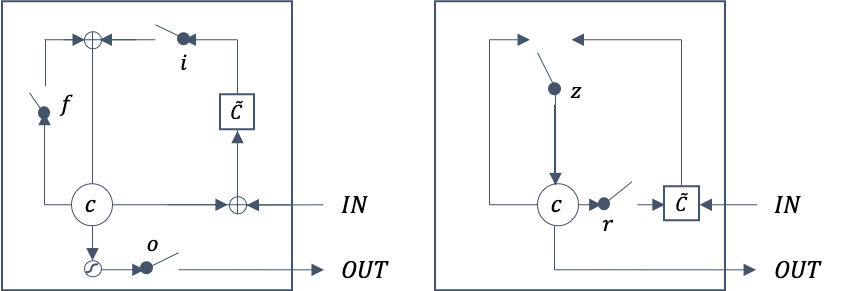
\includegraphics[scale=0.7]{fig13.png}
  \caption{RNN vs GRU}
  \label{fig:16-13}
\end{figure}

위의 그림은(\ref{fig:16-13}) 앞선 도식들과 달리 시간의 흐름에 따른 전파가 아닌, Input과 Output 관점에서 LSTM와 GRU의 셀을 회로도처럼 표현한 것이다. 왼쪽의 LSTM에서 세 개의 gate인 $f, i, o$가 스위치처럼 표현이 되어 있는 것을 알 수 있다. 반면, 오른쪽의 GRU 모델은 $z, r$이라는 스위치가 두 개만 존재함을 확인할 수 있으며 LSTM의 셀 상태(cell state)가 없는 대신 Hidden Information인 $h$가 위치하고 있다.

\begin{equation}
	\begin{split}
		z_t & = \sigma(W_z x_t + U_z h_{t-1} + b_z)\\
        r_t & = \sigma(W_r x_t + U_r h_{t-1} + b_r)\\
        \tilde{h}_t & = tanh(W_h x_t + U_h (r_t \odot h_{t-1}) + b_h)\\
        h_t & = (1-z_t) \odot h_{t-1} + z_t \odot \tilde{h}_t
	\end{split}
	\label{eq:16-12}
\end{equation}

Output $h_t$는 update gate인 $z$ gate를 통해 이전 시점의 Hidden information을 얼마나 유지하고, 현재 시점의 Hidden information을 얼마나 받아들일지를 결정하게 된다. LSTM에서 $i$ gate와 $f$ gate 에 의해서 결정되던 부분들이 GRU에서는 $z$ gate 하나로 결정된다라고 이해할 수 있겠다. $r$ gate는 이전 시점의 정보를 얼마나 현재 시점의 정보와 융합시킬지를 결정하는 gate로서 reset gate라고 불린다. 
 
% 3. -----------------------------------------------------------------
\section{RNN Based MNIST Classification}

% 3.1 -----------------------------------------------------------------
\subsection{Detour: MNIST Dataset}
RNN 계열의 뉴럴 네트워크를 응용할 수 있는 분류문제(Classification)를 다뤄보기 이전에 간략하게 MNIST 데이터셋에 대해서 짚어보도록 하겠다. MNIST 데이터 셋은 0에서부터 9까지의 손글씨를 모아놓은 데이터로 총 6만 개의 학습 데이터와 1만 개의 테스트 데이터가 있다. 하나의 데이터 샘플은 아래의 그림(\ref{fig:16-14})과 같이 흑백이미지로 구성이 되어 있는데, $28 \times 28$ 픽셀로 구성되어 있기 때문에 총 784개의 픽셀로 이루어져있다. MNIST데이터는 아래 그림(\ref{fig:16-15})와 같이 텐서플로우(Tensorflow)의 API에서 불러올 수 있다.

\begin{figure}[ht] \centering 
  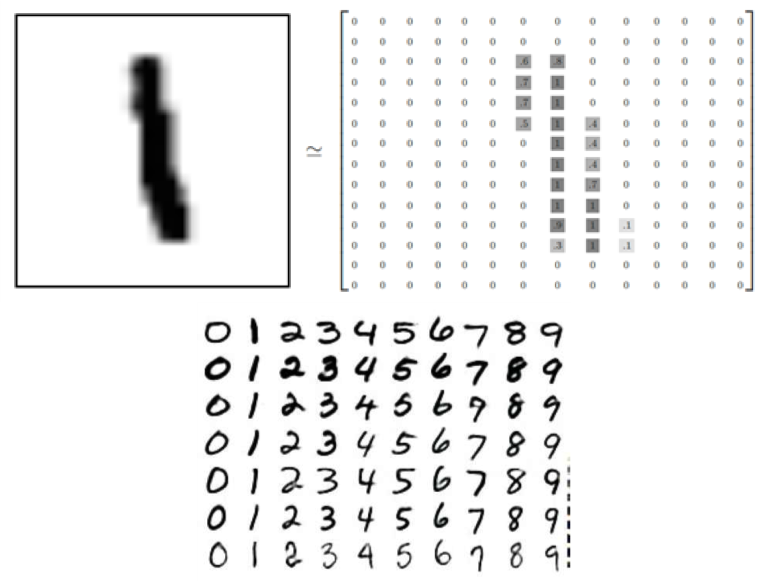
\includegraphics[scale=0.2]{fig14.png}
  \caption{MINST 데이터 샘플}
  \label{fig:16-14}
\end{figure}

\begin{figure}[ht] \centering 
  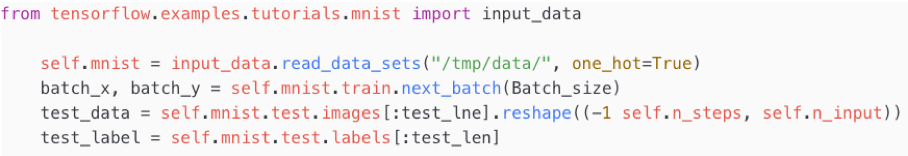
\includegraphics[scale=1.0]{fig15.png}
  \caption{Load MNIST dataset}
  \label{fig:16-15}
\end{figure}

MNIST 데이터셋의 분류 문제를 Convolution Neural Network(CNN)으로 수행을 한다고 하였을 때는 아래 그림(\ref{fig:16-16})과 같이 나타낼 수 있다. 즉, $28 \times 28$ 픽셀의 이미지가 입력값으로 주어졌을 때 특정 사이즈의 필터(fileter)가 이미지들을 훓어나가면서 합성곱(convolution)을 진행하게 된다. 이를 통해 더 작은 사이즈의 텐서(Tensor)형태로 줄여나가지면서 하나의 숫자로 만들어지는 네트워크 구조를 만들 수 있겠다. 이미지라는 데이터는 비슷한 정보들이 같은 지역에 모여져 있다는 특징이 있다. 따라서 CNN 구조는 이러한 이미지의 특징(locality)를 잘 반영할 수 있는 구조라할 수 있겠다. 다만 본 장에서는 RNN 계열의 네트워크를 다소 쉬운 문제에 적용해본다는 의미에서 이러한 MNIST 데이터의 분류 문제에 접근을 해보도록 하겠다.

\begin{figure}[ht] \centering 
  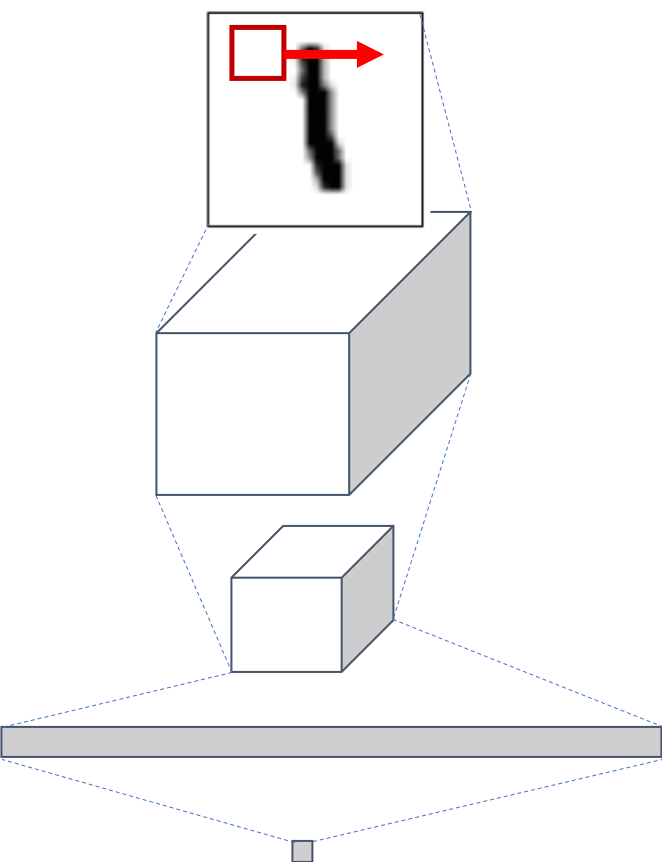
\includegraphics[scale=0.5]{fig16.png}
  \caption{CNN mnist classfication}
  \label{fig:16-16}
\end{figure}

% 3.2 -----------------------------------------------------------------
\subsection{MNIST Classification with RNN}
독자들은 공항 검색대에서는 비행기 탑승자들에게 금속 탐지기로 머리부터 발까지 스캔을 하는 모습을 보았을 것이다. RNN 계열의 네트워크 이용하여 이미지 분류를 할 때에는 이와 유사하게 데이터를 처리한다. 즉, 시간의 흐름에 따라 이미지 상단 행(row)부터 아래쪽 행(row)의 정보를 읽어나가도록 할 것이다. 따라서 한 시점에 입력되는 $1 \times 28$ 픽셀로 이루어진 데이터가 되고 28 타임스텝(time step)이 지나면 이미지의 모든 정보를 읽을 수 있게 된다. 행(row)으로 처리하는 것 이외에 하나의 픽셀로만 입력값을 구성할 수도 있다. 이 경우에는 28 타입스텝이 아니라 784 타임스텝이 필요하다. 물론, 이미지 데이터를 분석함에 있어 CNN보다는 위와 같은 방법들이 부적절하다고 볼 수 있으나 RNN 계열의 네트워크를 시험삼아 테스트하기에 충분하다고 볼 수 있겠다. 아래 그림(\ref{fig:16-17})은 하나의 층으로 이루어진 LSTM 네트워크로 마지막 상태(state)값 $h_{28}$을 이용하여 클래스를 나타낸다. 그러나 실제로는 잠재 정보 $h_t$를 이용하여 더 깊은 층을 쌓을 수도 있으며, RNN이나 GRU 셀을 이용하여 모델을 만들 수 있다.

\begin{figure}[ht] \centering 
  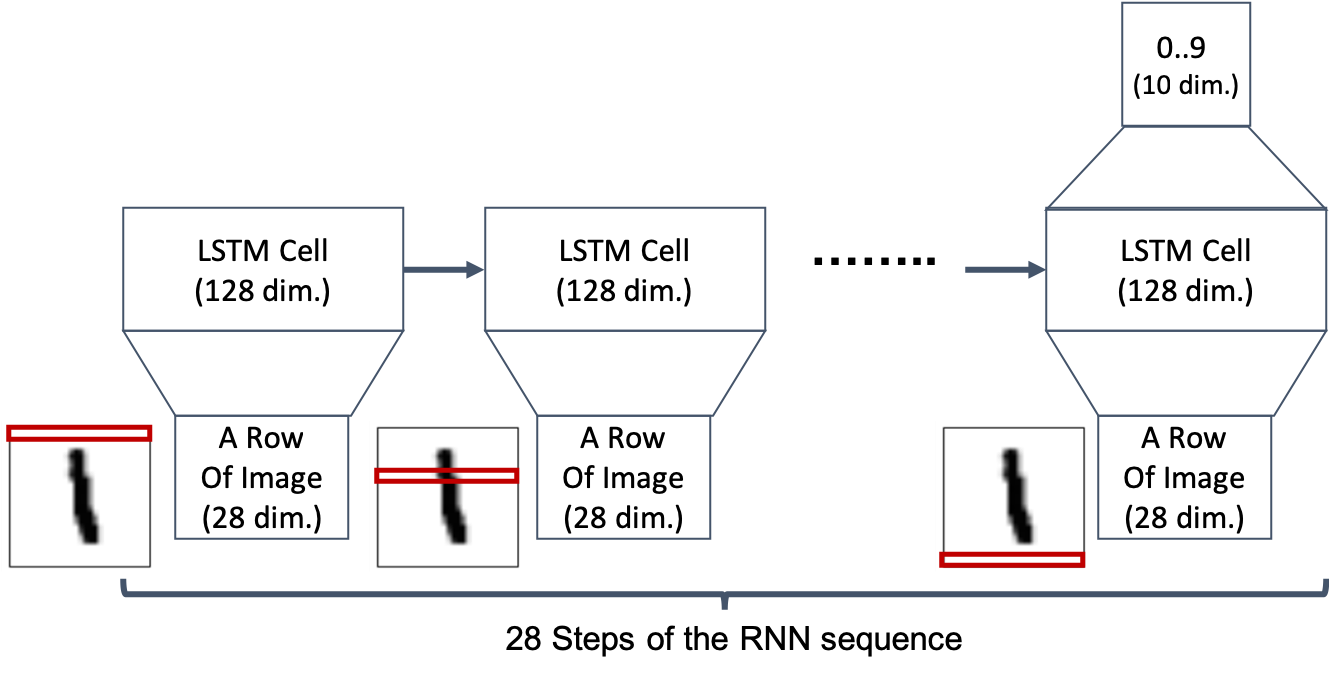
\includegraphics[scale=0.5]{fig17.png}
  \caption{MNIST classification with RNN}
  \label{fig:16-17}
\end{figure}

% 3.3 -----------------------------------------------------------------
\subsection{Tensorflow Implementation - RNN Structure}
텐서플로우(Tensorflow)의 텐서(Tensor)는 벡터(Vector)나 행렬(Matrix)를 보다 일반화한 개념이다. 따라서 0차원 (0 Rank) 텐서는 스칼라(Scalar), 1차원 텐서는 벡터, 2차원 텐서는 행렬(Matrix) 그리고 3차원 이상의 텐서(Tensor)  고차원 벡터를 가리킨다. 이러한 개념을 토대로 텐서플로우 API를 이용한 코드(\ref{fig:16-18})를 살펴보겠다.
\begin{figure}[ht] \centering 
  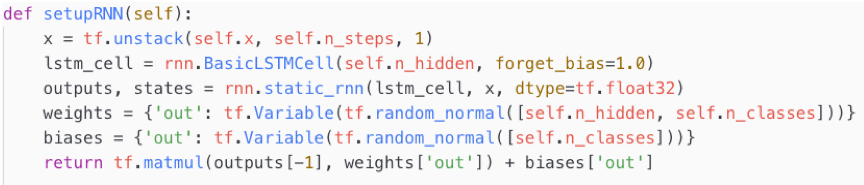
\includegraphics[scale=1.0]{fig18.png}
  \caption{Set up RNN}
  \label{fig:16-18}
\end{figure}

MNIST 이미지는 $28 \times 28$픽셀의 2차원의 이미지 데이터이지만, 실제 모델에 입력되는 값은 $1\times 28$의 1차원 정보가 들어가게 된다. 따라서 2차원 이미지 데이터를 28개의 1차원 데이터로 변환시켜주는 작업이 먼저 필요하다. 이것이 첫번째 줄의 \textit{tf.unstack} 함수가 하는 역할이다.  2차원인 이미지 x를 n\_steps(=28)만큼 1차원으로 잘라주는데 이것은 행을 기준(axis=1)으로 이루어진다.\par
그림(\ref{fig:16-17})에서도 나와 있듯이 LSTM 셀에서 잠재 정보는 128 차원으로 이루어져 있다. 따라서 두번째 줄의 \textit{rnn.BasicLSTMcell} 함수에서 128개의 h\_hidden을 명시하여 셀을 정의한다. 그림(\ref{fig:16-17})에서는 마치 28개의 LSTM 셀이 있는 것처럼 보이지만, 앞에서도 학습했듯이, 사실은 하나의 셀이 동일한 parameter를 이용하여 28 스텝동안 데이터를 처리한다. 세번째 줄의 \textit{rnn.static\_rnn} 함수는 위에서 정의해준 lstm\_cell을 주어진 타임스텝만큼 이용될 수 있도록 한다. 마지막으로 \textit{weights}와 \textit{biases}를 \textit{outputs[-1]}(마지막 잠재 정보 $h_{28}$)과 fully connect하여 최종 클래스를 반환하게 된다.

% 3.4 -----------------------------------------------------------------
\subsection{Tensorflow Implementation - Learning Mechanism}
앞에서는 모델 구현에 대해서 알아보았고, 모델의 학습을 위해서는 Backpropagation이 필요하다. 텐서플로우를 통하여 모델 학습 과정이 어떤 식으로 이루어지 아래의 코드를 통해 확인해보도록 하겠다.

\begin{figure}[ht] \centering 
  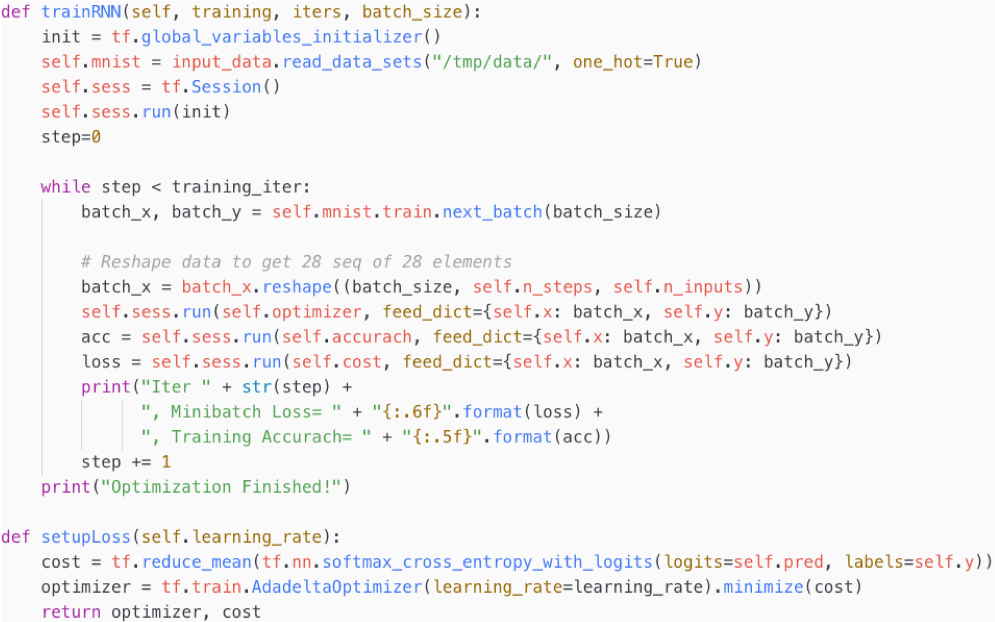
\includegraphics[scale=1.0]{fig19.png}
  \caption{Train and Set up Optimization}
  \label{fig:16-19}
\end{figure}

텐서플로우의 오퍼레이션(operation)은 \textit{tf.sess}라는 클래스에 의해서 이루어진다. \textit{sess} 객체를 통해서 변수에 대해서 초기화를 하거나 학습을 위해 데이터를 입력하고 출력값을 받아낼 수 있다. 네번째 줄에서 \textit{sess} 멤버 함수 중 \textit{run}을 실행시키는데, 이는 모델을 구성하는 변수들을 초기화 하는 과정이 포함되어 있다. 초기화는 \textit{tf.global\_variables\_initializer} 등과 같은 함수를 이용할 수 있다. \par
아래의 \textit{while loop}구문 내부가 실제 학습을 하는 과정을 담고 있다. 앞에서 알아보았듯이 텐서플로우 API를 통해 MNIST데이터셋을 불러올 수가 있고, \textit{next\_batch} 함수를 통해 지정된 배치사이즈(batch size)만큼 나누어 이미지 데이터(\textit{batch\_x})와 그에 대응하는 라벨(label, \textit{batch\_y})를 반환한다. 이때, \textit{batch\_x}는 784개의 픽셀로 이루어진 1차원 벡터로 이루어져 있기 때문에 \textit{tf.reshape}함수를 이용해서 2차원 이미지($28 \times 28$)로 바꾸어 준다. 따라서 \textit{batch\_x}는 [\textit{batch\_size} $\times$ 784]에서 [\textit{batch\_size} $\times$ 28 $\times$ 28]인 형태로 바뀌게 된다. 그리고 두번째 \textit{sess.run}에서는 위에서 만들어진 \textit{batch\_x}와 \textit{batch\_y}를 딕셔너리(dictionary) 자료형태로 모델에 넘겨주게 된다. \par
여기서 optimizer는 아래쪽의 \textit{setupLoss}라는 함수에 정의되어 있다. Cost함수는 크로스 엔트로피(Cross Entropy)를 줄여서 오차를 줄이도록 하고 있다. 그리고 Gradient 방법 중의 하나인 Adam을 \textit{tf.train.AdamOptimizer} 함수를 사용하여 간편하게 사용할 수 있다. \par
위 코드에 사용된 함수에 관하여 더욱 자세한 설명은 텐서플로우의 도큐멘테이션(Documentation)을 참조하기 바란다. 

% 4. -----------------------------------------------------------------
\section{Attention Network}

% 4.1 -----------------------------------------------------------------
\subsection{Overview}
기본적으로 Attention Network가 없더라도 RNN은 작동한다. 그러나 좀 더 나은 효과를 내기 위해서 덧붙여지는 네트워크 중 하나가 Attention Network이다. Attention Network를 설명하기 위해 시간의 흐름에 따라 'I am a boy' 라는 문장이 입력된다고 가정해보자. 이제까지 자연어 처리 분야(NLP, Nature Language Process)에서는 통상적으로 관사인 a를 제거하곤 했다. 그러나 이를 완전히 제거하지는 않되, 관사를 주의(Attention)깊게 보지 않는 네트워크가 더 나은 성능을 보일 수 있다. 혹은 'It is a beautiful flower.'라는 문장에서 'beautiful'이 핵심적인 내용을 담고 있다고 가정해보자. 그렇다면 우리가 모델링하는 네트워크는 'beautiful'에 보다 더 많은 주의(Attention)를 기울여야만 한다. 그러나 기존의 RNN 계열의 구조에서는 입력되는 각각의 값들이 동일한 비중으로 받아들여진다. 따라서 시점에 따라 입력되는 값들에 각기 다른 가중치를 부여하여 네트워크를 만들 수 있게 하는 것이 Attention Mechanism이라고 할 수 있겠다. 이러한 Attention Mechanism는 image captioning, object detection, 추천 시스템(recommender system)에서 사용된다. 

% 4.2 -----------------------------------------------------------------
\subsection{Attention Structure}

\begin{figure}[ht] \centering 
  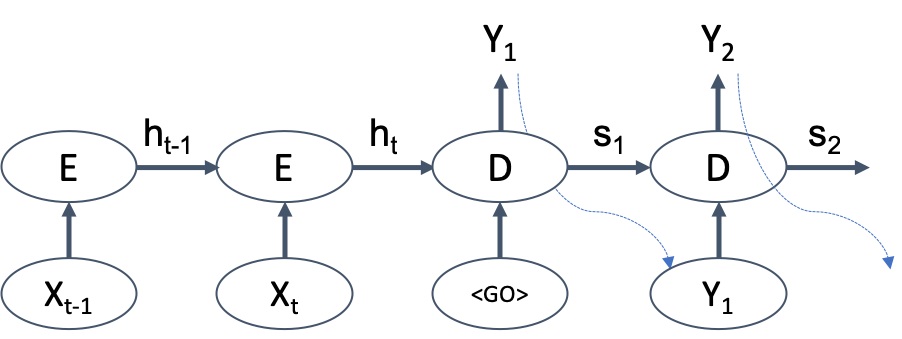
\includegraphics[scale=0.6]{fig20.png} 
  \caption{Encoder-Decoder Network}
  \label{fig:16-20}
\end{figure}

\begin{equation}
	\begin{split}
		h_i & = f(x_i, h_{i-1})\\
		c & = q(h_1, ..., h_T)\\
	\end{split}
	\label{eq:16-13}
\end{equation}

위의 그림(\ref{fig:16-20})과 같이 RNN 계열의 네트워크로 Encoder-Decoder 네트워크를 구성한다고 생각을 해보자. $f$와 $q$를 뉴럴 네트워크와 같이 비선형의 함수라고 가정하고, $c$는 주어진 $x = (x_1, ..., x_T)$를 함축하는 정보(context) 라고 하자. Encoding 단계에서 주목해야하는 것은 $h_T$는 1) $x_T$의 임베딩(embedding)으로서 역할과 2) $h_1, ..., h_T$를 포괄하는 정보를 담는 역할을 가지게 된다 라는 점이다. 그러나 만약 두 번째 역할로 인하여 $h_T$를 $c$라고 할 경우에는 $c = q(h_1, ..., h_T) = h_T$가 되어버리므로 $h_1, ..., h_{T-1}$에 해당하는 정보는 소실되어 버리게 된다. 따라서 $h_T$는 첫 번째 역할만을 수행하면서, $h_T$의 두번째 역할을 담당할 수 있는 $c$를 잘 정의할 필요가 있다.\par

\begin{equation}
	P(y) = \prod_{i=1}^{T}P(y_t|t_1, ..., y_{t-1}, c)
	\label{eq:16-14}
\end{equation}

Decoding단계에서는 이점 시점의 정보들과 Context $c$를 사용하여 위의 수식(\ref{eq:16-14})과 같이 나타낼 수 있다. 이와 같은 구조에서 확률 분포는 뉴럴 네트워크를 통해서 아래(\ref{eq:16-15})와 같이 모델링할 수 있겠다. Context $c$를 만들어내야 하는 이유가 밝혀졌으니, 다음 절에서 $c$를 어떤 식으로 정의할 수 있는지를 학습해보도록 하자. 

\begin{equation}
	P(y_t|t_1, ..., y_{t-1}, c) = g(y_{t-1}, s_t, c)
	\label{eq:16-15}
\end{equation}

% 4.3 -----------------------------------------------------------------
\subsection{Attention Structure Definition}
시간이 흘러감에 따라 입력되는 모든 입력값들의 context를 담고 있는 $c$와 개별 시점에서 얻게 되는 지역적인 $c_t$ 중 어떤 것이 위에서 제시된 Attention Mechnism을 보다 효과적으로 구현해낼 수 있을까? 예컨대 '나는 점심을 먹었다.'라는 문장을 영어로 바꿔야 된다고 생각해보자. 'I had lunch.' 라는 번역된 문장에서 'I'라는 단어를 예측을 할 때 $c$보다는 개별 시점에서 얻어진 $\{c_1, c_2, c_3\}$ 중 $c_1$만을 활용하여 예측을 하는 것이 더 높은 성능을 보일 수 있을 것이다.  즉, Decoding 단계에서 각 시점에 필요한 context는 Encoding 단계에서의 일부 시점의 context라고 할 수 있겠다. 따라서 위와 같은 아이디어를 반영한 결과가 아래 수식(\ref{eq:16-16})이라고 할 수 있겠다.

\begin{equation}
	\begin{split}
		P(y_t|t_1, ..., y_{t-1}, c_t) & = g(y_{t-1}, s_t, c_t)\\
		s_t & = f(s_{t-1}, y_{t-1}, c_t)
	\end{split}
	\label{eq:16-16}
\end{equation}

이전에 $c$를 도입하였을 때 일부 $s_t$와 $c$의 관계가 모호하였던 것에 반하여, 새롭게 정의된 수식에서는 이 관계가 명확해진다. 현재 시점 $t$에서의 context $c_t$와 이전 시점의 입력값 $y_{t-1}$과 잠재 정보(hidden information)인 $s_{t-1}$을 이용하여 현재 시점의 잠재 정보 $s_t$를 생성하게 된다. 즉, Encoder에서 시점마다 만들어진 context 정보인 $c_t$를 이용하여 Decoder에서 각 시점의 hidden information인 $s_t$를 만들 수 있는 함수 $f$가 필요하게 된다. 그럼 Encoder에서 $c_t$는 어떻게 만들어질 수 있을까?\par

\begin{equation}
	\begin{split}
		c_l & = \sum_{i=1}^{T}\alpha_{l,i} h_i\\
	\end{split}
	\label{eq:16-17}
\end{equation}

특정 시점 $l \in \{1, 2, ..., T\}$의 context $c_l$은 총 시간 $T$ 동안 Encoder에 의해서 생성되는 모든 잠재 정보 $h_i$에 $\alpha_{l,i}$라는 가중치를 부여한 값의 합으로 구할 수 있다. 이 $\alpha_{l,i}$는 앞에서 살펴본 바와 같이 각 시점에서 어떤 부분을 주의(attention)깊게 보고, 어떤 부분은 주의깊게 보지 않을지를 결정하는 가중치라고 할 수 있겠다. 앞선 예제를 다시 떠올리면, 'I'라는 단어를 예측하기 위해서는 '나는'이라는 단어에 더 큰 가중치를 둔다. 반면 'lunch'라는 단어를 예측하기 위해서는 '점심'이라는 단어에 더 큰 가중치를 두는 역할을 $\alpha$가 수행하게 된다. 다만 $T$가 길어지면 길어질수록 이 가중치들의 합은 계속해서 커지기 때문에, 정규화(Normalized)된 값을 사용하게 된다. \par

\begin{equation}
	\begin{split}
		\alpha_{l,i} & = \frac{\exp{(e_{t,i})}}{\sum_{k=1}^{T}\exp{(e_{l,k})}}\\
        e_{l,i} & = a(s_{l-1}, h_i)
	\end{split}
	\label{eq:16-18}
\end{equation}

위의 수식(\ref{eq:16-18})에서 Softmax의 모양을 지닌다는 것을 알 수 있는데, 마치 다항분포에서 어떤 클래스를 선택할지에 대한 문제와 유사한 형식을 가진다. 따라서 여러 가지 단어들이 개별 클래스가 되고 이 단어들 중에서 하나의 값을 취하는 문제로 바뀌게 된다. Softmax function 내부에 필요한 alignment $e_{l,i}$은 Scoring Mechanism으로 바라 볼 수 있다. 이는 Encoder와 Decoder에서 생성되는 잠재 정보 사이의 유사도를 측정하여 결정된다. Alignment에서 사용되는 $a$라는 함수는 뉴럴 네트워크로 만들 수도 있거나, 혹은 Encoder와 Decoder의 결과값 사이에 같은 척도(metric)가 사용된다면 단순하게 유클리디안 거리(Euclidean Distance)나 코사인 유사도(Cosine similarity)를 사용할 수 있을 것이다.
    
% 4.3 -----------------------------------------------------------------
\subsection{Global Attention Structure}

\begin{figure}[ht] \centering 
  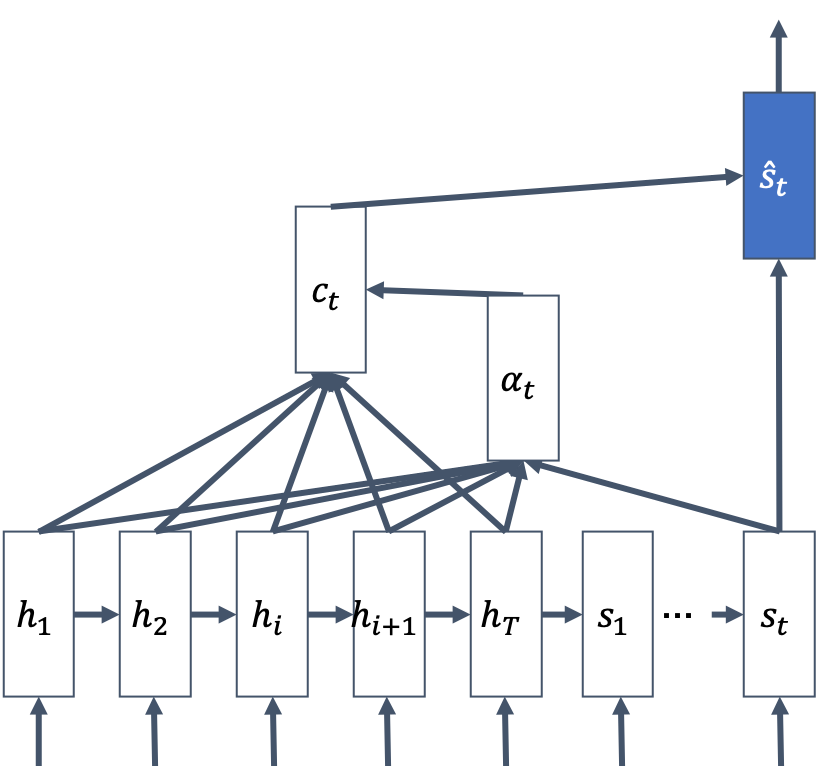
\includegraphics[scale=0.5]{fig21.png} 
  \caption{그림 2:23}
  \label{fig:16-21}
\end{figure}

위의 그림(\ref{fig:16-21})을 통해 앞서 학습하였던 Attention Mechanism이 어떻게 작동하는지 알아보겠다. 현재 시점 $t$에서 우리가 관심있는 것은 Encoder에서 전달되는 context 정보인 $c_t$를 반영한 $\hat{s}_t$를 구하는 것이다. 이를 위해 필요한 정보는 이전 시점의 $y_{t-1}$, $s_{t-1}$과 $c_{t}$이다. 그림(\ref{fig:16-21})에서 가중치 $\alpha_{t,l}$는 Encoder의 모든 잠재 정보 $h_1, h_2, ..., h_T$와 각각 비교하여 만들어진다. 이를 다시 수식으로 나타내어 보자면 아래와 같다. 

\begin{equation}
	\alpha_{t,i} = \frac{\exp{(a(s_t, h_i))}}{\sum_{k=1}^{T}\exp{(a(s_k, h_k))}}
	\label{eq:16-19}
\end{equation}

재차 언급하지만 $a$는 임의의 함수라도 사용이 가능하므로 어떤 함수 $a$로 설계를 할 것인지도 하나의 연구 분야가 될 수 있을 것이다. $\alpha_{t}$는 총 $T$개의 벡터로 이루어져 있고, 이 값들의 합은 1이 됨을 앞에서 배웠다. 이후 Encoder의 각 시점마다 가중치 $\alpha_{t,i}$를 반영하여 합한 결과가 $c_t$가 된다는 것을 알 수 있다. 이는 또다시 아래의 식(\ref{eq:16-20})으로 표현된다.

\begin{equation}
	c_t = \sum_{i=1}^{T}\alpha_{t,i}h_i
	\label{eq:16-20}
\end{equation}

그리고 우리가 관심있었던 $\hat{s}_t$는 context 벡터인 $c_t$와 현재 시점의 잠재 정보 $s_t$와 연결(concatenated)되어 아래(\ref{eq:16-21})와 같이 구해진다. 

\begin{equation}
	\hat{s}_t = tanh(W_c[c_t; s_t])
	\label{eq:16-21}
\end{equation}

이렇게 보면 Attention Mechanism에 대한 overivew에서 제기되었던 문제점이 더욱 잘 와닿을 수 있을 것이다. 기존 RNN 계열의 모델에서는  $h_T$가 $c_t$나 $\alpha_t$가 하는 역할을 모두 담당했다라고 볼 수 있다. 따라서 추가적인 Attention Structure의 도입으로 $h_T$의 정보만 의존하지 않으면서 보다 나의 성능을 기대할 수 있게된 셈이다. 그러나 많은 경우에 그러하듯, Attention Mechanism 역시 장점뿐만 아니라 단점을 지니고 있다. Attention Mechanism은 Decoder의 매 시점마다 T번의 alignment, context벡터, 그리고 $\hat{s}_t$의 계산 과정을 거쳐야만 한다. 따라서 더 나은 성능을 위한 비용이 크다라는 단점이 존재한다. 따라서 이러한 단점을 해결하기 위해서 제안된 것이 전체 시간 T를 보지않고 지역적인 부분만을 고려하자는 것이다. 

% 4.3 -----------------------------------------------------------------
\subsection{Local Attention Structure}

\begin{figure}[ht] \centering 
  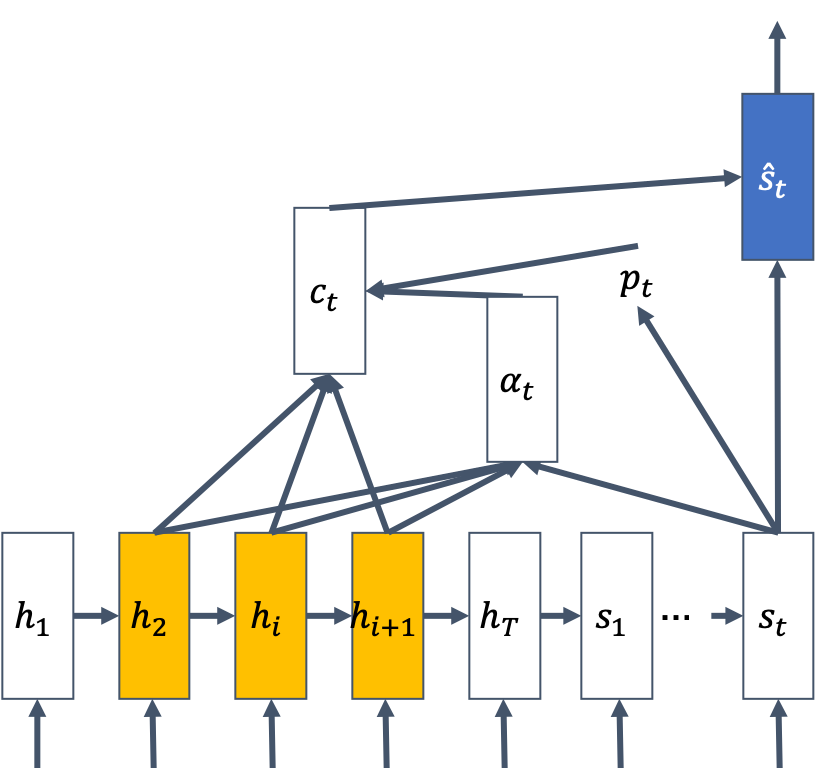
\includegraphics[scale=0.5]{fig22.png} 
  \caption{그림 2:23}
  \label{fig:16-22}
\end{figure}

Local Attention Structure을 쉽게 이해하기 위해서 GP(Gaussian Process)를 떠올려 보도록 하자. GP에서 전체 시간을 고려하지 않고, window size만큼의 moving average만을 고려하였다. 이 때 kernel(i.e. RBF kernel $k(x, x_i) = \exp{(-\frac{|x-x_i|^{2}}{2\sigma^{2}})}$)을 이용해서 window size 안에서도 가중치를 달리하여 중요도를 변화시켜 보았다. GP와 유사하게 Local Attention Structure는 Encoder의 전체 sequence의 특정 시점 $p_t$에서 $D$만큼의 시간만 고려하여 Attention Mechanism을 적용하게 된다.

\begin{equation}
	\begin{split}
		c_t & = \sum_{i=p_t - D}^{p_t + D}\alpha_{t,i}h_i\\
        \alpha_{t,i} & = \frac{\exp{(e_{t,i})}}{\sum_{k=p_t - D}^{p_t + D}\exp{(e_{t,k})}}\exp{(-\frac{(i-p_t)^{2}}{2(\frac{D}{2})^{2}})}\\
        e_{t,i} & = a(s_t, h_i)
	\end{split}
	\label{eq:16-22}
\end{equation}

수식(\ref{eq:16-20})에서 window size가 $2d$인 moving window를 적용한 수식이 위의 수식(\ref{eq:16-22})이라고 할 수 있겠다. $c_t$를 구할 때 전체 sequence $T$가 아닌 특정 시점 $p_t$의 전후의 $D$만큼의 시점만 포함하고 그 너머로는 고려하지 않겠다라는 것을 확인할 수 있다. 뿐만 아니라 $\alpha_{t,i}$에서 RBF와 유사하게 Bell shaped curve로 window 내부에서도 가중치를 변경시키도록 한다. 그러나 어느 위치를 기준으로 바라보아야 할까에 대한 의문이 들게 되는데 이는 새로운 네트워크를 이용하여 해결해줄 수 있다.

\begin{equation}
	\begin{split}
		p_t & = T \times \sigma(v_{p}^{T}tanh(W_p s_t))
	\end{split}
	\label{eq:16-23}
\end{equation}

즉, 현재 시점 $t$의 잠재 정보(Hidden information) $s_t$에서 변수 $W_p$와 $tanh$을 이용해 네트워크를 구성하고 새로운 가중치 $v_p$를 도입하여 계산을 할 수 있다. 그리고 Logistic function과 같이 Sigmoid function $\sigma$를 통해 0과 $T$사이의 점을 선택할 수 있다. 하지만 한국어와 영어처럼 주술 구조가 반대로 된 경우에는 $p_t$에서 window 크기만큼을 바라본다는 것은 정보 누락의 위험이 다소 크다고 볼 수 있다. 그럼에도 불구하고 이 구조에서 $p_t$가 pointer로서 특정 대상에 대한 위치를 예측할 수 있다는 것은 중요한 점이라 할 수 있겠다. 예컨대 '철수는 영희를 만났다. 그녀는 그의 친구이다.'라는 문장에서 대명사인 '그녀'와 '그'가 가리키(point)는 대상인 '철수'와 '영희'를 $p_t$로 가리킬 수만 있다면 Decoder 단계에서 보다 다양하게 이를 활용할 수 있을 것이다. 
\end{document}
